\documentclass[oneside,a4paper]{article}

% ========== Preamble (packages, definitions etc.) ==========

\usepackage[utf8]{inputenc}
\usepackage[english]{babel}
\usepackage{graphicx}
\usepackage{xcolor}
\usepackage{amsmath, amsthm, amssymb}
\usepackage{csquotes}
\usepackage{hyperref}
\usepackage{listings}
\usepackage{lmodern}
\usepackage[explicit]{titlesec}
\usepackage{color}
\usepackage{listings}
\lstset{
    breaklines=true,
    basicstyle=\tt\normalsize,
    keywordstyle=\color{blue},
    identifierstyle=\color{magenta},
    frame = single
} 
\definecolor{redbg}{RGB}{235, 214, 214}
\definecolor{Red}{RGB}{163, 25, 25}
\definecolor{Black}{RGB}{0, 0, 0}


\titleformat{\section}
  {\normalfont\LARGE\bfseries}
  {}
  {0em}
  {\colorbox{redbg}{\parbox{\dimexpr\textwidth-2\fboxsep\relax}{\textcolor{Red}{\thesection\quad#1}}}}

\titleformat{\subsection}
  {\normalfont\large\bfseries\color{Black}}
  {\thesubsection}
  {1em}
  {#1}
  [{\titlerule[0.8pt]}]

\titlespacing\subsection{0pt}{12pt plus 4pt minus 2pt}{0pt plus 2pt minus 2pt}
%\usepackage[backend=bibtex,style=abbrv]{biblatex}
\newcommand{\todo}[1]{{\color{blue}#1}}  % show to-do items in blue
\setlength{\parskip}{\baselineskip}
\usepackage[activate={true,nocompatibility},
            final,
            tracking=true,
            kerning=true,
            %spacing=nonfrench,
            factor=1100,
            stretch=10,
            shrink=10,
            nopatch=eqnum]{microtype}
%\hypersetup{
%    pdftitle={},
%    bookmarks=true,
%    pdfpagemode=FullScreen,
%}

\newcounter{questionnum} \setcounter{questionnum}{0}
%\newcommand{\question}[1]{%
%  \refstepcounter{questionnum}%
%  \paragraph{Question~\arabic{questionnum}:}{\emph{#1}}}

\newcommand\filltoend{\leavevmode{\unskip
  \leaders\hrule height.5ex depth\dimexpr-.5ex+0.4pt\hfill\hbox{}%
  \parfillskip=0pt\endgraf}}

\newcommand{\problem}[2]{%
	\vspace{-0.7em}
	\hspace{0.02\textwidth}
	\begin{minipage}[t][][b]{0.95\textwidth}
		{\bf \hspace{-0.015\textwidth}\makebox[7.5em][l]{{#1} ~~\filltoend}}%
		\hspace{1.2mm}{\it #2}%
	\end{minipage}
}

\def\email#1{{\tt#1}}

\lstset{ % Set the default style for code listings
	numbers=left,
	numberstyle=\scriptsize,
	numbersep=8pt,
	basicstyle=\scriptsize\ttfamily,
	keywordstyle=\color{blue},
	stringstyle=\color{red},
	commentstyle=\color{green!70!black},
	breaklines=true,
	frame=single,
	language=bash,
	tabsize=4,
	showstringspaces=false
}
\usepackage{svg}
\usepackage{float}
\usepackage[margin=2cm]{geometry}
\usepackage{pdfpages}
\usepackage[title]{appendix}
\usepackage{indentfirst}
\usepackage{caption, subcaption}
\usepackage{enumitem}


% ========== Title page ==========

\title{
	
\includegraphics[width=0.6\textwidth]{UU_logo.pdf}\\[1em]
	Computer-Assisted Image Analysis I - 1TD396\\[1em]
	Computer Exercise 3\\[3em]
}

\author{
	Jyong-Jhih Lin, \and Linus Falk, \and Niklas Kostrzewa, \and Teng-Sung Yu
	%
}

\date{November 23, 2022}

\begin{document}

\maketitle
\thispagestyle{empty} % Removes page number for front page
\pagebreak

% ========== Document contents ==========

\section{Introduction}
In this assignment we are asked to count the number of coins in a provided image. 

\section{Method}
Below is a Matlab script that solves the problem of counting coins (and classifiying them) presented. Each method is commented why its needed in the script.

\begin{lstlisting}[language=MATLAB]
I=imread('lab3_material/coins.tif');
x`subplot(2,3,1)
imshow(I) %Display input image

f=[1 1 1 1; 1 1 1 1; 1 1 1 1; 1 1 1 1;]./16; %filter small sharp edges on coin surface
I=imfilter(I,f,'symmetric');
I = medfilt2(I); %Filer bright pixels.
T = graythresh(I); % Find treshold to mask away background
I_2 = im2bw(I,T);   % create binary image of background and coins

%figure(1)
subplot(2,3,2)
imshow(I_2) %Display binary image


%figure(3)
subplot(2,3,3) 
Idist = bwdist(I_2,"euclidean"); %Calculate distance to edges
Idist = -Idist; %invert it for the next step
se = strel('disk',5);
Idist = imerode(Idist,se);  % try to remove small not connected parts of coins
imshow(Idist,[]);


%figure(5)
subplot(2,3,4)
L = watershed(Idist); %watershed to isolate each coin after eroding
L(I_2) = 0; %set background to zero
rgb = label2rgb(L,'spring',[1 1 1]);
imshow(rgb)

%figure(6)
subplot(2,3,5)
T = 0;
I_2 = im2bw(L,T); % create a new binary image with all coins separated
imshow(I_2)

%figure(7)
subplot(2,3,6)
Ilabel=bwlabel(I_2,4); % label all objects, coins in the binary image


stats = regionprops('table',I_2,'Centroid','MajorAxisLength','MinorAxisLength'); %get properties, center and majoraxis length
centers = stats.Centroid;
diameters = stats.MajorAxisLength;
radii = diameters/2;
imshow(I_2)
hold on
viscircles(centers,radii); %display all objects radii with circles, centered with majoraxis length
title('Radii','Interpreter','latex', 'fontsize',22)
hold off

figure(9)
radii(radii < 17) = []; % remove small objects befor making histogram
hist(radii, 30)

figure(8)
F=regionprops(Ilabel,'Area');
A=[F.Area];
A(A<200) = []; 
hist(A)
title('Area','Interpreter','latex', 'fontsize',22)
\end{lstlisting}

\newpage 

\section{Result}

\begin{figure}[ht!]
\centering
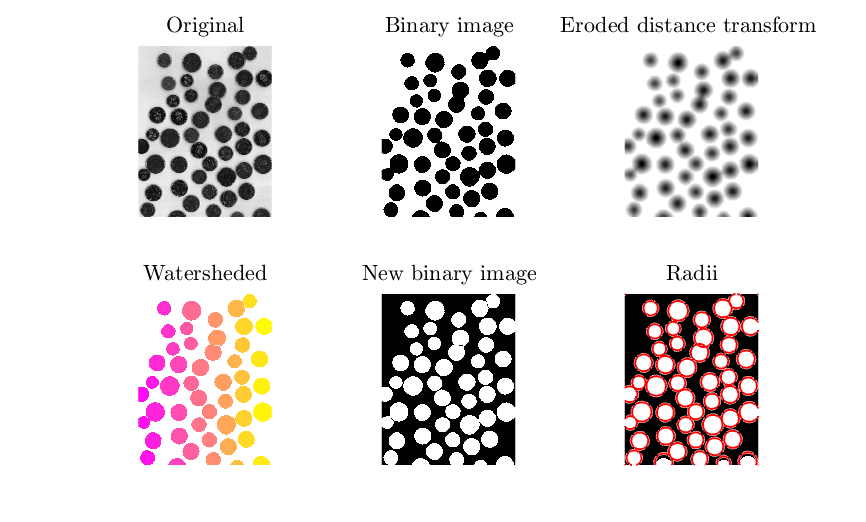
\includegraphics[width=130mm]{figures/assign_3.png}
\caption{Example of caption}
\label{fig:workprocess}
\end{figure}

\begin{figure}[ht!]
\centering
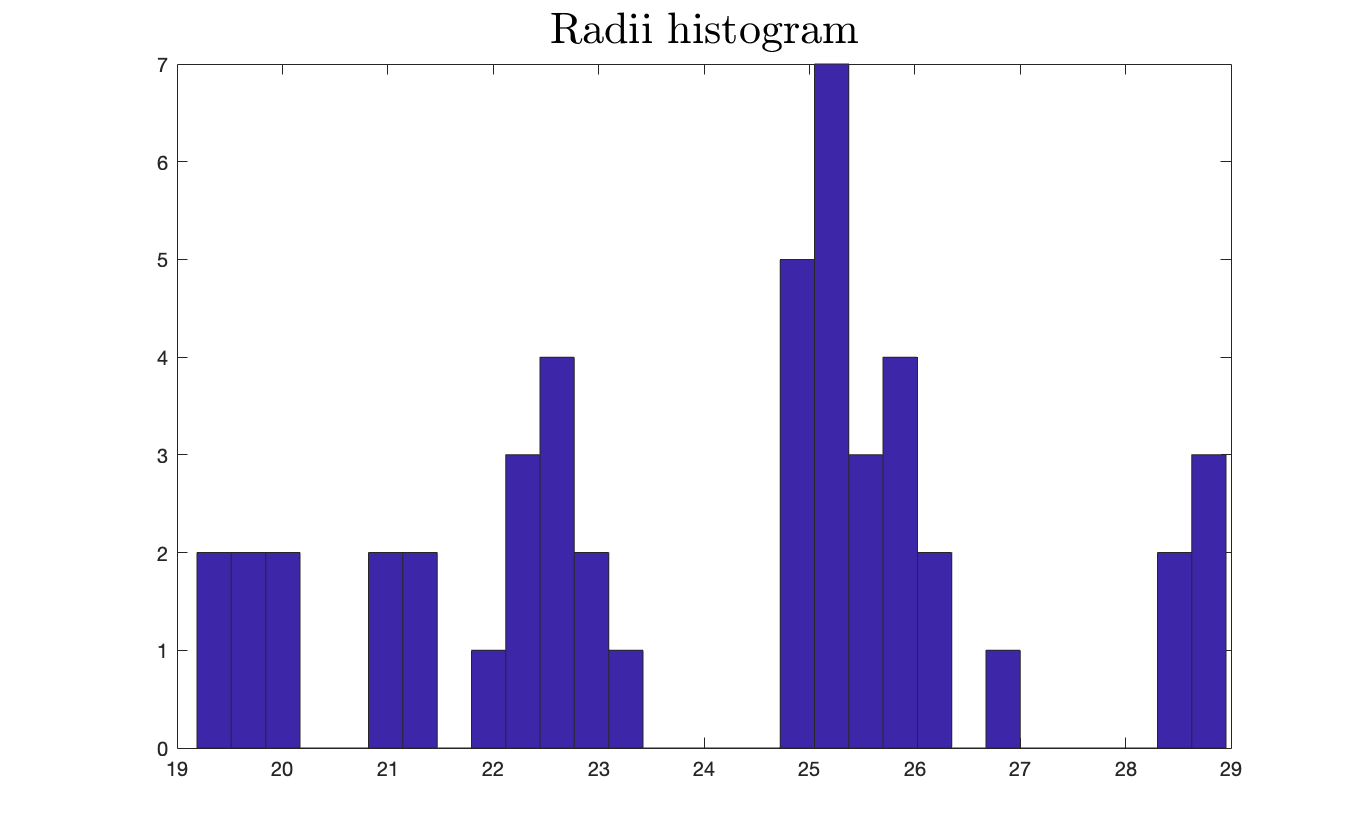
\includegraphics[width=100mm]{figures/assign_3b.png}
\caption{Example of caption}
\label{fig:result}
\end{figure}


\section{Discussion}

\noindent \textbf{A discussion of errors and limitations in your final method.}

The method can count all coins in the image but have problem with classifying one of the coins. Better pre-processing to avoid shadows being included as edge of the coin could be one solution. On order to correctly classify half of the coin most be in the image. 

\noindent \textbf{As you can see, the objects are coins. Is it possible to count the total amount
of money using your algorithm?}

It is possible to count the sum of the money. More compex allgorithm would be needed if less then half of the coin is present in the image to correctly classify it with radius. In this model the objects longest axis is used to calculate the radii, by doing this we can approximate the radius and get a good classification of the partial image of the coins. 


\noindent \textbf{Explain how your method treat the coins on the image border.}

As described above is the majoraxis lenght used to identify the radii of the coins which works well as long as at least half the coin is in the image. 



\noindent \textbf{Is your solution general in the sense that it can be used when analyzing im-
ages with arbitrary circular objects (i.e. not only coins.tif)?}

Taking the bacteria image as an example. It is possible to count the number of bacteria in the image depending on how you define \textbf{one} bacteria. In the image we can see several bacteria during \textbf{binary fission/mitosis(?)}, when during this process do we consider it to be a new bacteria? There is some problem with "dirt" in the image but most of it can be "filtered" out in the classification by setting the threshold size correct.  

\begin{figure}[ht!]
\centering
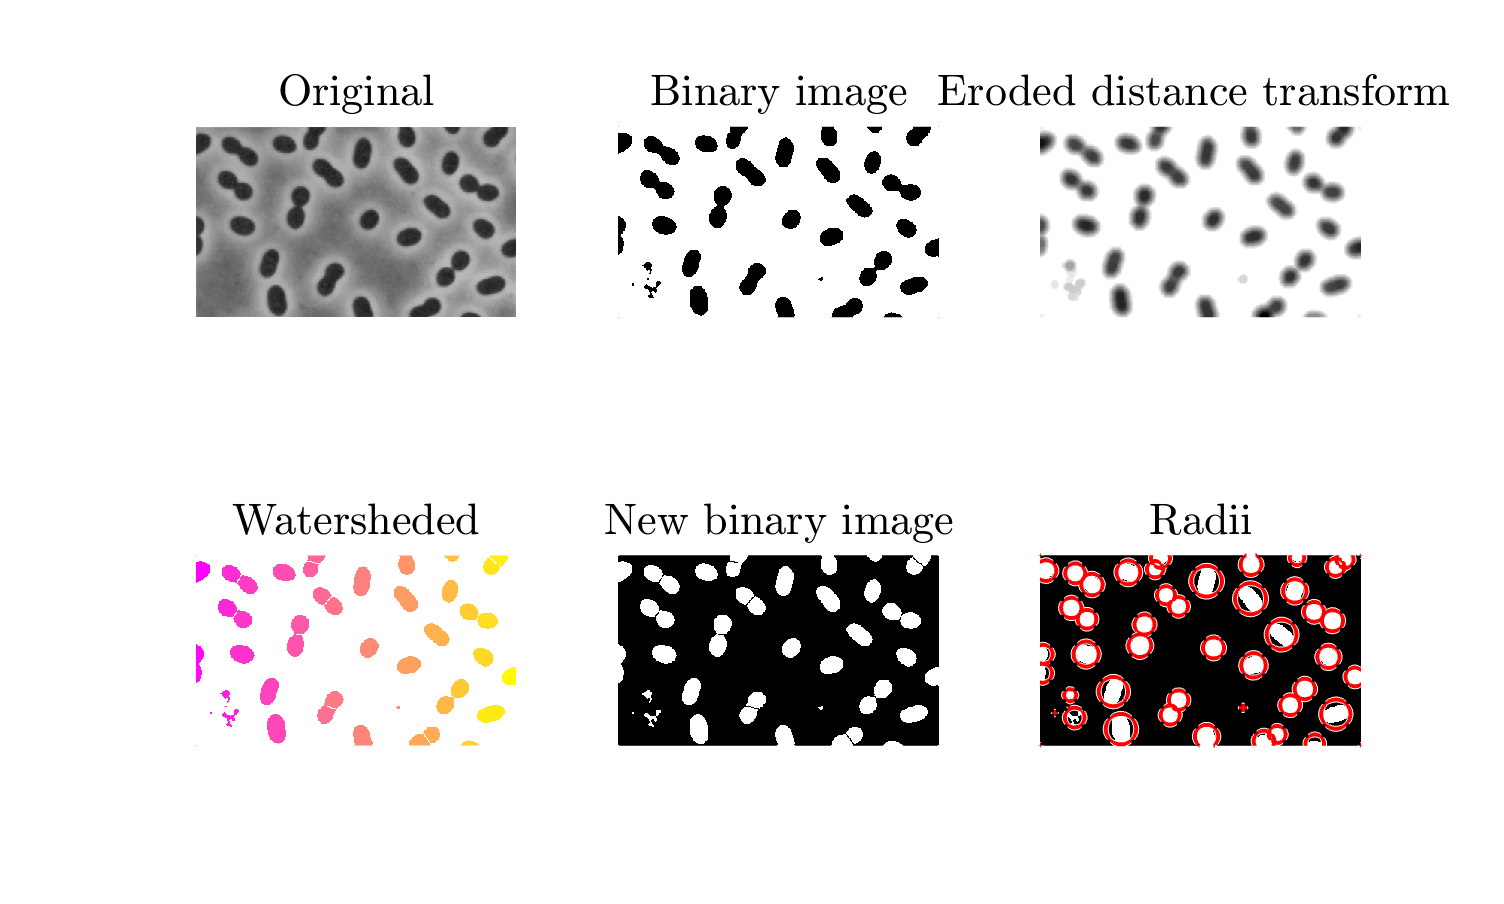
\includegraphics[width=130mm]{figures/assign_3c.png}
\caption{}
\label{fig:workprocessbac}
\end{figure}

\begin{figure}[ht!]
\centering
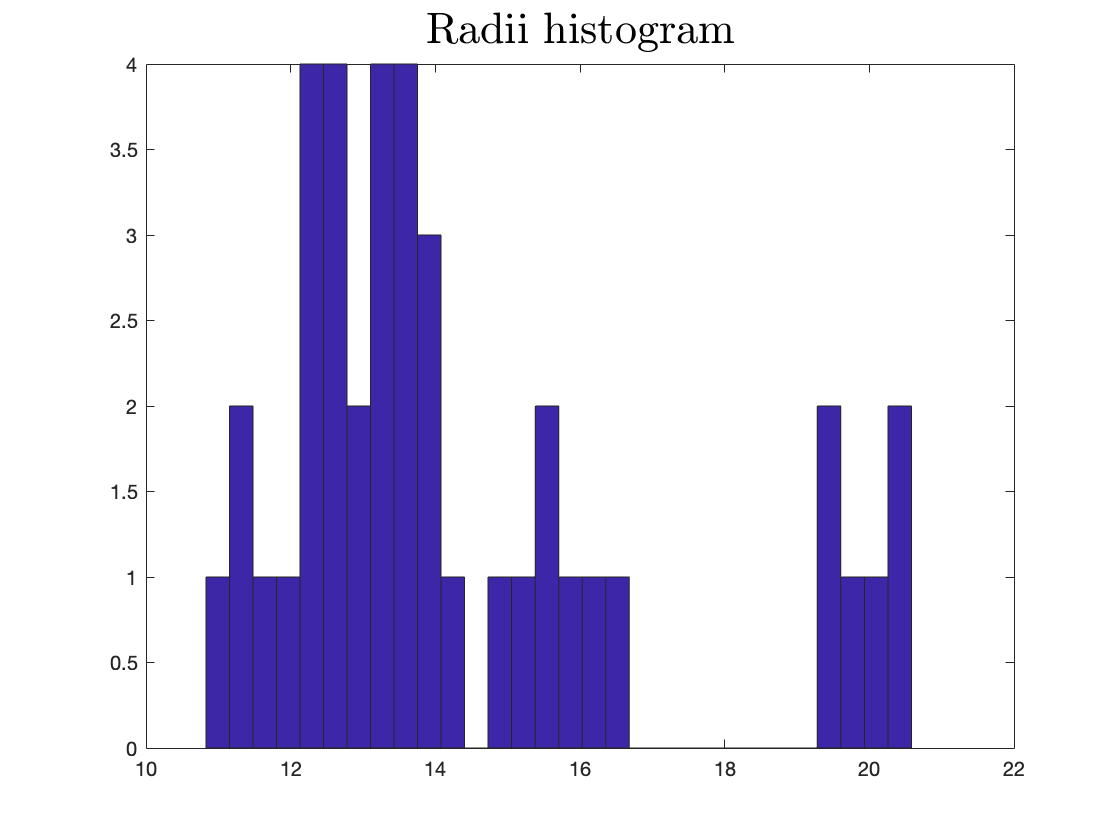
\includegraphics[width=100mm]{figures/assign_3d.png}
\caption{}
\label{fig:resultbac}
\end{figure}











% Delete this section if you have no plot to submit.
% Change the size of the figure by changing the value in [width=300pt]

% Putting \autoref{fig:my_figure} in your text will refer to the corresponding figure label.
% Eg.: "\autoref{fig:my_figure} clearly shows that the large circle is larger than the small box."
% Read more about autoref here https://en.wikibooks.org/wiki/LaTeX/Labels_and_Cross-referencing#autoref

%\bibliographystyle{apalike}
%\bibliographystyle{abbrv}
%\bibliography{bibliography}

\end{document}